\documentclass[twocolumn]{iopjournal}

\usepackage{amsmath,amssymb,amsfonts}
\usepackage{array}

\fancyhfoffset[L]{0mm}
\setlength{\marginparwidth}{0pt}
\setlength{\marginparsep}{0pt}

\renewcommand{\articletype}[1]{%
  {\vspace*{-8mm}\noindent \Large \sf Preprint}\par
  \vspace*{6mm}\noindent{\scriptsize \sf{\bfseries \MakeUppercase{#1}}}}

\fancyhead[L]{}
\fancyhead[R]{}

\hypersetup{pdftitle={The Affine Connection of the Tiled Cube}, pdfauthor={Stephen Nelson}, pdfsubject={Gravity Field Dynamics (GFD)}, pdfkeywords={affine connection, torsion, Christoffel symbols, tetrad, stellated octahedron, tiling, vortex, proof}}

\begin{document}

\articletype{Proof}

\title{The Affine Connection of the Tiled Cube}

\author{Stephen Nelson}

\affil{Field Dynamics Research}

\ead{stephen@fielddynamics.org}

\begin{abstract}
The affine connection $\Gamma^\lambda{}_{\mu\nu}$ has 64 components
because each of its three indices runs over four values, and
general relativity keeps the 40 symmetric in $\mu\nu$ and sets the
24 antisymmetric ones, the torsion, to zero. Neither the count nor
the discarded part is usually given a geometric meaning. We give
both. Gravity Field Dynamics works with a cube holding a stellated
octahedron, and cubes tile space. Each face of the cube's
tetrahedron TetA is cut into four channels, and in the tiling each
channel is shared by exactly four cubes, so each face carries 16
couplings and the tetrahedron 64. We prove that these 64 couplings
correspond one-to-one with the connection's index triples, respecting
every symmetry, with one role per index: the face is $\lambda$, the
channel is $\mu$ and the leg of the tetrad along which the coupled
cube lies is $\nu$. The dictionary is a formula in the tetrad's legs,
forced once the roles are fixed, and under it the couplings split
exactly as the Christoffel ($40$) and torsion ($24$) sectors do.
Torsion then has a plain meaning on the tiles: it is the handedness
of the couplings, made of a circulation around each face and a flow
along each leg, in which the core's couplings reach across to the
TetB side. With the tiling's closure rule nothing crosses from TetA
to TetB; without it, exactly the 24 couplings that carry the
circulation do. A torsion-free connection is a tiling whose couplings
have no handedness.
\end{abstract}

\keywords{affine connection, torsion, Christoffel symbols, tetrad, stellated octahedron, tiling, vortex, proof}

% ----------------------------------------------------------------------

\section*{Why this proof}

The connection tells a field how to change from one place to the
next. In general relativity it has $K^3 = 64$ components, and the
torsion-free condition keeps $40$ and discards $24$ by convention.
Letter~2 showed that the discarded $24$ are the only place a
connection can tell the tetrad equation's two roots, TetA and TetB,
apart~\cite{NelsonL2,NelsonGram}, and the torsion proof that they
form the regular representation of the legs' permutations, the one
home of the sign representation~\cite{NelsonTorsion}. What was
missing is a picture: why each index runs over four values, and what
the $24$ are, in space.

The framework's answer is the cube. Each cube holds one whole
stellated octahedron, TetA and TetB meeting in the Field Origin, and
cubes tile space~\cite{NelsonL1,NelsonTiling}. This proof shows that
the tiling builds the connection by itself. Nothing is added: the
$64$ are the ways the cube's faces are shared with its neighbours,
each index is a piece of that sharing, and the torsion is the part
of it that has a handedness, a swirl and a flow, as in a drained
vortex. General relativity is then the tiling with the handedness
removed.

\section*{The picture}

Look at one face of the cube's TetA. The TetB corner behind it
pierces it, cutting it into a small central triangle, the
\emph{core}, which is a face of the Field Origin, and three corner
triangles, which are faces of TetA's spikes: four channels, as in
Letter~1~\cite{NelsonL1,NelsonHalf}. In the tiling each corner
channel faces one of the octahedra that fill the space between
stars, and each such octahedron is held jointly by the four cubes
around a cube edge. The core faces the three neighbouring cubes
whose Field Origins touch it at its corners. So every channel is
shared by four cubes: $4 \times 4 = 16$ couplings per face, four
faces, $64$. Figure~\ref{fig:tiles} shows one face and one shared
octahedron.

\begin{figure*}[t]
\centering
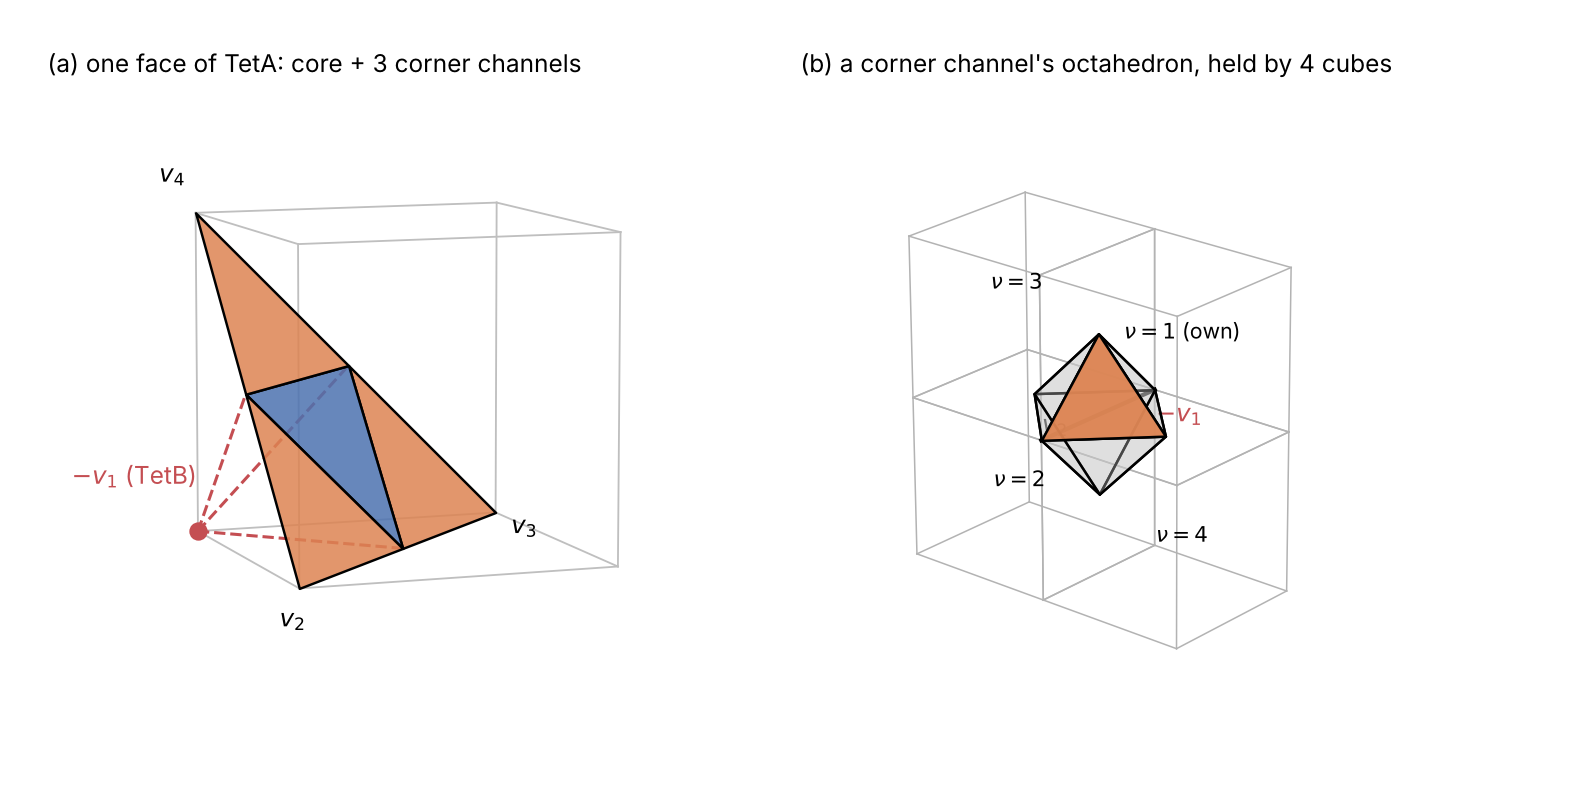
\includegraphics[width=0.92\textwidth]{tiled_cube_figure.png}
\caption{(a) The face of TetA opposite $v_1$, cut by the TetB corner
$-v_1$ (red; dashed, the TetB spike standing on the core) into the
core (blue), a face of the Field Origin, and three corner channels
(orange), faces of TetA's spikes. (b) The corner channel at $v_2$
(orange) is a face of the octahedron on the cube edge from $v_2$ to
$-v_1$, which is held by four cubes, one along each leg $\nu$ from
$-v_1$: the cube itself ($\nu = 1$), the cube diagonally across
($\nu = 2$) and two face neighbours ($\nu = 3, 4$). Drawn by
\texttt{make\_figure.py} from the same coordinates as the checks.}
\label{fig:tiles}
\end{figure*}

Each coupling is a channel of a face reaching a neighbouring cube,
and the neighbour lies along one of the tetrad's four legs. Face,
channel, leg: three indices, each running over four values. That is
$\Gamma^\lambda{}_{\mu\nu}$.

% ----------------------------------------------------------------------

\section*{Setting and premises}

The cube centred at $2n$, $n \in \mathbb Z^3$, has side $2$; write a
cube by its centre. The forced frame's legs $v_1, \dots, v_4$ are the
corners of $[-1,1]^3$ with $xyz = +1$~\cite{NelsonForced,NelsonGram},
with
\begin{equation}
  \textstyle\sum_a v_a = 0, \qquad v_a \cdot v_b = 4\delta_{ab} - 1 .
  \label{eq:frame}
\end{equation}
TetA is the tetrahedron on the $v_a$, TetB the one on the $-v_a$,
and the Field Origin their intersection, the octahedron
$|x| + |y| + |z| \le 1$. The face of TetA opposite $v_\lambda$ is
pierced by the TetB corner $-v_\lambda$. Its channel $\mu$ is the
core for $\mu = \lambda$ and the corner triangle at $v_\mu$ for
$\mu \neq \lambda$, the half-space proof's own labels~\cite{NelsonHalf}.
$T_d$ denotes the 24 symmetries of the cube keeping TetA; it acts on
the legs as $S_4$~\cite{NelsonGram}.

\paragraph{(T) Tiling.} Cubes tile space, each holding one whole
stellated octahedron.

\paragraph{(S) Sharing.} A channel couples to a cube when that cube
shares it: when the channel is a face of an octahedron the cube helps
hold, or when it touches the cube's Field Origin. Nothing couples at
a distance; this is the Laplacian's neighbour comparison.

\medskip\noindent
(S) names the framework's two routes between cells. The vortices
proof has the same two: a corner channel couples spatially, through
the solid on its far side, and the core gravitationally, through the
Field Origin~\cite{NelsonVortex}. The rule is applied the same way to
every channel. A corner channel's two corners at cube-face centres
also touch Field Origins, but only those of cubes already holding its
octahedron, so both routes give the same four cubes (check~2.6). The
one contact (S) leaves out is the spike tip, the cube corner, which
all eight cubes around it touch. A tip is neither Field Origin nor a
shared octahedron, and the vortices proof's cube graph bonds a corner
only inward, to its own cube's Field Origin~\cite{NelsonVortex}.
Counting that contact would give $4 + 3 \times 8 = 28$ couplings per
face (check~2.7). A shared octahedron does run along a cube edge,
from a TetA corner to a TetB corner, which is the bond the vortices
proof leaves out. It is not added here: a coupling joins a channel to
a cube, never one corner to another.

\paragraph{(C) Closure.} Where cubes meet they agree: every shared
corner carries one chamber, TetA or TetB, in all eight cubes
around it~\cite{NelsonI,NelsonTiling}. Only Theorem~6 uses (C):
Theorems~1--5 use (T) and (S) alone and hold for any labelling of the
tiling. In this proof ``closure'' means (C) only.

\medskip\noindent
A \emph{coupling} is a pair (channel of a face of TetA, cube sharing
it).

\paragraph{Index roles.} In the dictionary below, $\nu$ is the
direction (the leg along which the coupled cube lies) and $\mu$ is
what is carried (the channel), so that
$\Gamma^\lambda{}_{\mu\nu}$ reads as
$\theta^\lambda(\nabla_{e_\nu} e_\mu)$. The order of the two lower
indices differs across the literature: Carroll and Hawking--Ellis put
the direction first~\cite{Carroll,HawkingEllis}. The two orders
differ by $\mu \leftrightarrow \nu$, which leaves the $40/24$ split
unchanged and reverses the sign of the torsion. Signs of torsion
components below follow the torsion proof's
$t_{a;bc} = (a,b,c) - (a,c,b)$~\cite{NelsonTorsion}.

% ----------------------------------------------------------------------

\section*{Theorem 1 (the honeycomb)}

\emph{The star fills half its cube: its eight spikes and the Field
Origin. The other half is twelve wedges, one on each cube edge, each
a quarter of an octahedron. Around each edge the four cubes' wedges
close into one octahedron, its eight faces spike faces, two from
each cube. So the cubes fill space with stars and shared octahedra in
equal volume.}

\paragraph{Proof.} In units of the small tetrahedron the cube is
$24$, a spike $1$ and an octahedron $4$: $8 + 4 = 12$, and the rest
is $12$ quarter octahedra. That the four wedges around each edge
close into one octahedron, two faces from each cube, is checked face
by face at every interior edge of a $3 \times 3 \times 3$ block
(check~1.2; also~\cite{NelsonTiling}). \hfill $\square$

% ----------------------------------------------------------------------

\section*{Theorem 2 (every channel is shared by four cubes)}

\emph{For the face of TetA opposite $v_\lambda$:}
\begin{enumerate}
\item[(i)] \emph{its core is shared by the cube and by the three face
  neighbours at $-v_\lambda - v_p$, $p \neq \lambda$;}
\item[(ii)] \emph{its corner channel $\mu \neq \lambda$ is a face of
  the shared octahedron centred at the cube-edge midpoint
  $(v_\mu - v_\lambda)/2$, which runs from the TetA corner $v_\mu$ to
  the piercing TetB corner $-v_\lambda$, and is shared by the four
  cubes around that edge;}
\item[(iii)] \emph{so each channel is shared by exactly four cubes,
  each face carries $16$ couplings and TetA carries $64 = K^3$, and
  the face reaches seven of the eight cubes around $-v_\lambda$.}
\end{enumerate}
\emph{The core channels together couple the cube to each of its six
face neighbours exactly twice.}

\paragraph{Proof.} (i) The core's corners are the cube-face centres
$(v_q + v_r)/2$, $q, r \ne \lambda$, which~(\ref{eq:frame}) rewrites
as $-(v_\lambda + v_p)/2$ with $p$ the face's third corner. A face
centre $f$ is a corner of the Field Origins of the cubes at $0$ and
$2f$. (ii) By~(\ref{eq:frame}) $v_\mu \cdot v_\lambda = -1$, so
$v_\mu$ and $-v_\lambda$ differ in one coordinate and
$(v_\mu + v_\lambda)/2$ is a unit vector. The corner triangle's
vertices $v_\mu$ and $(v_\mu + v_q)/2$ are then the edge midpoint
$(v_\mu - v_\lambda)/2$ plus unit vectors: they are vertices of the
octahedron there, which Theorem~1 shares among four cubes. (iii)
Counting, and the two TetA faces of the Field Origin through each
cube-face centre. \hfill $\square$

% ----------------------------------------------------------------------

\section*{Theorem 3 (the dictionary)}

\emph{The four cubes sharing channel $\mu$ of face $\lambda$ are
centred at}
\begin{equation}
\begin{aligned}
  c_{\lambda\mu\nu} &= -v_\lambda + \varepsilon_{\lambda\mu\nu}\,v_\nu,\\
  \varepsilon_{\lambda\mu\nu} &=
  \begin{cases} +1 & \nu \in \{\lambda, \mu\},\\ -1 & \text{otherwise,}\end{cases}
\end{aligned}
  \label{eq:dict}
\end{equation}
\emph{one along each leg $\nu$ from the piercing TetB corner. Hence}
\begin{equation}
  (\lambda, \mu, \nu) \;\longmapsto\;
  (\text{channel } \mu \text{ of face } \lambda,\ \text{cube } c_{\lambda\mu\nu})
  \label{eq:map}
\end{equation}
\emph{is a bijection from the $64$ index triples onto the $64$
couplings, and it commutes with $T_d$. It is forced: of the $1152$
bijections that commute with $T_d$, it is the only one in which
$\lambda$ is the face, $\mu$ the channel and $\nu$ a leg from
$-v_\lambda$, and of the 32 symmetric sign rules only
$\varepsilon$ gives the couplings. TetB obeys~(\ref{eq:dict}) with its
own legs $-v_a$, and parity carries one dictionary to the other index
for index.}

\paragraph{Proof.} For $\mu = \lambda$, Theorem~2(i) gives the cubes
$0 = -v_\lambda + v_\lambda$ and $-v_\lambda - v_p$. For
$\mu \ne \lambda$, the four cubes around the edge at
$(v_\mu - v_\lambda)/2$ are $0$, $v_\mu - v_\lambda$ and, since
the legs sum to zero, $-v_\lambda - v_q$, $-v_\lambda - v_r$
(Theorem~1): the cases
$\nu = \lambda$, $\nu = \mu$ and the other two legs. Distinct $\nu$
give distinct cubes, since the legs and their negatives are eight
distinct corners, so~(\ref{eq:map}) is injective, hence bijective.
It is built from the legs alone, so $T_d$, which permutes them,
commutes with it. The cubes around $-v_\lambda$ are
$-v_\lambda \pm v_\nu$, which leaves one choice of $\nu$ for each
coupling once the channel is fixed. The counts of bijections and of
sign rules are by enumeration. \hfill $\square$

\medskip\noindent
Each channel thus couples along all four legs of the tetrad. A face
is a $4 \times 4$, channels by legs, a copy of the tetrad frame, and
the four faces are the four slices of the connection. In general
relativity each factor of four is the number of coordinates; here
each is a piece of geometry.

% ----------------------------------------------------------------------

\section*{Theorem 4 (the sectors)}

\emph{Under $T_d$ the $64$ couplings fall into orbits of sizes
$4, 12, 12, 12, 24$, as the index triples do, with character
$(64, 8, 1, 0, 0)$ on the classes $e$, $(12)$, $(123)$, $(1234)$,
$(12)(34)$, that of $V \otimes V \otimes V$. Exchanging the lower
indices, $\mu \leftrightarrow \nu$, splits them into}
\begin{itemize}
\item \emph{an even part, $40$ dimensions, isomorphic as a
  representation of $T_d$ to the Christoffel sector
  $V \otimes \mathrm{Sym}^2V$, namely
  $4\cdot\mathbf 1 \oplus 3V_2 \oplus 7\,\mathrm{std} \oplus
  3(\mathrm{sgn}\otimes\mathrm{std})$~\cite{NelsonB};}
\item \emph{an odd part, $24$ dimensions, isomorphic to the torsion
  sector $V \otimes \Lambda^2V$, the regular
  representation~\cite{NelsonTorsion}.}
\end{itemize}
\emph{The sign representation occurs once, in the odd part. The
Field Origin is the row $\mu = \lambda$ of each slice, and the
diagonal $\mu = \nu$ is each channel's coupling straight along its
own leg: the core to its own cube, a corner channel through its
shared octahedron to the cube diagonally across.}

\paragraph{Proof.} The bijection~(\ref{eq:map}) commutes with $T_d$,
so the orbits and characters are those of the triples; the
multiplicities follow by orthogonality of characters, computed on
the traces of $g$ and of $g\tau$, $\tau$ the exchange. The last
sentence reads~(\ref{eq:dict}) at $\mu = \lambda$ and $\mu = \nu$.
\hfill $\square$

\medskip\noindent
The slice structure is the Gram proof's index grid, six upper, four
diagonal and six lower entries per slice~\cite{NelsonGram}; the
theorem says which coupling each entry is.

% ----------------------------------------------------------------------

\section*{Theorem 5 (torsion is the couplings' handedness)}

\begin{enumerate}
\item[(i)] \emph{Mirror symmetry. On the $24$ couplings whose three
  indices differ, the corner channels' couplings to face neighbours,
  $\mu \leftrightarrow \nu$ is exactly the reflection exchanging legs
  $\mu$ and $\nu$. A torsion-free connection is mirror-symmetric
  there, and torsion is the couplings' handedness. On the other $24$
  with $\mu \ne \nu$ no symmetry maps a coupling to its partner.}
\item[(ii)] \emph{The torsion basis $t_{a;bc} = (a,b,c) - (a,c,b)$.
  Its incident half, $t_{a;ab}$, is the core's coupling to a face
  neighbour minus a corner channel's coupling to its own cube. Its
  non-incident half is the difference of two mirror-image corner
  couplings.}
\item[(iii)] \emph{Swirl. The totally antisymmetric torsion
  $\omega^a{}_{bc} = \sum_d \varepsilon_{abcd}$, which spans the sign
  representation, lives only on the corner channels' couplings to face
  neighbours, $+1$ for one sense of circulation around each face and
  $-1$ for the other. It is unchanged by rotations and reversed by
  reflections: a circulation.}
\item[(iv)] \emph{Flow. The vector torsion along leg $b$,
  $\sum_a t_{a;ab}$, pairs each core's coupling to the face neighbour
  at $-v_a - v_b$, on the $-v_b$ side, with a corner channel's
  coupling to its own cube. Its weights sum to zero, so its net
  displacement, $-2v_b$, does not depend on the origin: a flow along
  the leg, a polar vector. Its sign is the index convention's (the
  other order reads $+2v_b$); what does not depend on it is that the
  core's couplings reach across to the TetB side while the corner
  couplings paired with them stay home.}
\item[(v)] \emph{The swirl has no net displacement and the flow no
  support where the swirl lives. Torsion's vector part ($4$) lies on
  the incident couplings, its axial part ($4$) on the non-incident
  ones, and its tensor part is the remaining $16$, eight in each
  half.}
\end{enumerate}

\paragraph{Proof.} (i) For $\lambda, \mu, \nu$ distinct, the
reflection $\sigma$ exchanging $v_\mu$ and $v_\nu$ fixes $v_\lambda$
and sends $c_{\lambda\mu\nu}$ to $c_{\lambda\nu\mu}$
by~(\ref{eq:dict}). (ii)--(v) read~(\ref{eq:dict}) on the stated
tensors~\cite{NelsonTorsion}; the sense of circulation is the face's
rotation orbit. In (iv) the weights are $+1$ on the three cores'
couplings and $-1$ on three own-cube couplings, at $0$, so the
displacement is $\sum_{a \ne b}(-v_a - v_b) = -2v_b$
by~(\ref{eq:frame}), whatever the origin. \hfill $\square$

% ----------------------------------------------------------------------

\paragraph{Remark (the vortex reading).} Each face's swirl turns about
that face's own leg $v_\lambda$, and the four balance. Both facts are
forced by symmetry: the face's rotations fix only the axis
$v_\lambda$, and the legs sum to zero. Any quantity built to measure
the swirl, such as $\sum \omega\,(r_{\rm channel} \times c)$, points
along $v_\lambda$. Its size depends on where in the channel $r$ is
placed, so no size is claimed. What is not a matter of symmetry is
where the swirls sit. TetA's swirl on its face opposite $v_\lambda$
reaches cubes on the $-v_\lambda$ side, TetB's on its face opposite
$-v_\lambda$ reaches cubes on the $+v_\lambda$ side, and, a
circulation being an axial vector that parity keeps, the two turn
the same way: one swirl along each axis, TetA at one end and TetB at
the other, through the Field Origin (checks 5.13--5.14, for channels
placed at their centroids or at their spike tips). With the flow of
(iv) along the same leg, this is the shape of a drained vortex, a
swirl about an axis with a flow into the drain (the Burgers vortex
of the tug-of-war proof~\cite{NelsonTug}), and of the framework's
vortex, spiral, throat, spiral~\cite{NelsonVortex}. The reading is
the framework's; the algebra under it is exact.

% ----------------------------------------------------------------------

\section*{Theorem 6 (closure keeps the swirl inside TetA)}

\emph{Under (C), every neighbour reached through a shared octahedron
meets that octahedron with its own TetA at the same end as the cube
does, so no coupling crosses from TetA to TetB. If instead every cube
is labelled alike, the couplings that cross are exactly the $24$ with
three different indices: the corner channels' couplings to face
neighbours, the ones on which the swirl $\omega$ lives.}

\paragraph{Proof.} Under (C) a corner's chamber is the same in all
eight cubes around it, so the end $v_\mu$ of the octahedron of
Theorem~2(ii) is TetA for all four holders. Under the uniform
labelling the cube diagonally across, at $v_\mu - v_\lambda$, sees
$v_\mu$ at its own position $v_\lambda$, a TetA corner, while a face
neighbour at $-v_\lambda - v_\nu$ sees it at
$v_\mu + v_\lambda + v_\nu = -v_\rho$, $\rho$ the fourth leg, a TetB
corner, by~(\ref{eq:frame}). By the
dictionary these face neighbours are the $\nu \notin \{\lambda,\mu\}$
cases, the triples with all indices different, the support of
$\omega$ (Theorem~5(iii)). Checks 6.1--6.2. \hfill $\square$

\medskip\noindent
Given (C), the first sentence is immediate. The content is the
contrast: the labelling decides whether the handed couplings stay in
TetA, and closure is what keeps them there. This is not the torsion
subspace itself, which is a set of differences of couplings, not a
set of couplings.

% ----------------------------------------------------------------------

\section*{Necessity of the premises}

\vspace{4pt}
\noindent
{\footnotesize
\begin{tabular*}{\columnwidth}{@{\extracolsep{\fill}}l>{\raggedright\arraybackslash}p{0.74\columnwidth}@{}}
\hline
Removed & What fails \\
\hline
(T) & An isolated cube: each channel couples only to its own cube, $16$ couplings, not $64$ \\
(S) & Without sharing as the coupling rule the four cubes per channel, and so~(\ref{eq:dict}), have no source; counting every point of contact instead, the spike tips included, gives $28$ per face, not $16$ \\
roles & $1152$ bijections commute with $T_d$; the symmetry alone does not fix the dictionary \\
$\varepsilon$ & Each of the other $31$ symmetric sign rules misses the couplings \\
(C) & With every cube labelled alike, the face neighbours meet each shared octahedron with TetA at the other end: the $24$ couplings carrying the swirl cross into TetB \\
\hline
\end{tabular*}}
\vspace{4pt}

\noindent
Setting the torsion to zero is the converse: it removes the swirl and
the flow and keeps the mirror-symmetric $40$. This is the
torsion-free projection of the Gram proof, Theorem~3, read on the
tiles.

% ----------------------------------------------------------------------

\section*{What is proved and what is not}

Proved: the tiling's couplings correspond one-to-one with the
connection's index triples, by a forced, symmetric dictionary built
from the tetrad's legs; under it they split as the Christoffel and
torsion sectors do, the Field Origin is the row $\mu = \lambda$, and
torsion is the handedness of the couplings (a swirl and a flow);
closure is what keeps the handed couplings inside TetA. The vortex
through the Field Origin is a reading of these facts, with its
direction forced by symmetry.

Not proved:
\begin{enumerate}
\item \emph{Dynamics.} This is the connection's index structure,
  the level at which $\Gamma$ is built; its transformation law and
  parallel transport need a field on the tiling whose coupling
  coefficients are $\Gamma$. In such a field the torsion would be the
  net circulation through the corner channels; that is the next
  step.
\item \emph{Letter 2's reading of the $24$ as TetB.} The handed
  couplings are TetA's, and they run toward the TetB corner piercing
  each face (Theorem~2(ii)). Under the uniform labelling exactly the
  $24$ couplings carrying the swirl reach TetB (Theorem~6); under
  closure none does. Neither fact identifies the torsion subspace
  with TetB, so the reading is neither proved nor refuted here.
\item \emph{The $K^2$ of $a_0 = K^2Gm_e/r_e^2$.} Each face carries
  $K^2 = 16$ couplings; that this is the $K^2$ of $a_0$ is not shown.
\item \emph{Lean.} The statements are finite and integer; the
  formalisation is to follow.
\end{enumerate}

% ----------------------------------------------------------------------

\section*{Verification}

\texttt{verify\_tiled\_cube\_affine\_connection.py} runs $47$ exact
checks, numbered by theorem (check $i.j$ belongs to Theorem~$i$), in
integers and fractions with no floating point. The working notes,
with the two labellings of the tiling compared and the ladder of
$3 \times 3 \times 3$ blocks, are in
\texttt{research/diamond-tetrad-lattice/}\allowbreak\texttt{cube-tiling/}.

% ----------------------------------------------------------------------

{\small
\begin{thebibliography}{99}

\bibitem{NelsonL1}
S.~Nelson, \textit{The Coordinate-Space Geometry of the Tetrad Frame}
(Letter~1), Class.\ Quantum Grav.\ (2026), submitted (CQG-115428).

\bibitem{NelsonL2}
S.~Nelson, \textit{The Other Half of Gravity: Torsion and the
Two-Chamber Structure of the Tetrad Frame} (Letter~2), Class.\
Quantum Grav.\ (2026), submitted (CQG-115447).

\bibitem{NelsonHalf}
S.~Nelson, \textit{The Sixteen Half-Space Regions of the Tetrad Frame}
(2026), \texttt{proofs/half-space-two-bounded-regions/}.

\bibitem{NelsonForced}
S.~Nelson, \textit{The Spatial Geometry of the Lorentz Tetrad} (2026),
\texttt{proofs/forced-tetrahedral-frame/}.

\bibitem{NelsonGram}
S.~Nelson, \textit{The Gram Matrix of the Tetrad Equation} (2026),
\texttt{proofs/gram-matrix-tetrad-equation/}.

\bibitem{NelsonTorsion}
S.~Nelson, \textit{The Torsion Sector of the Tetrad Connection as the
Regular Representation of $S_4$} (2026),
\texttt{proofs/torsion-regular-representation/}.

\bibitem{NelsonB}
S.~Nelson, \textit{Torsion as the Regular Representation of $S_4$}
(Paper~B, 2026).

\bibitem{NelsonVortex}
S.~Nelson, \textit{Vortices of the Stellated Octahedron} (2026),
\texttt{proofs/vortices-of-the-}\allowbreak\texttt{stellated-octahedron/}.

\bibitem{NelsonTug}
S.~Nelson, \textit{The Constitutive Law as a Tug of War} (2026),
\texttt{proofs/constitutive-law-tug-of-war/}.

\bibitem{Carroll}
S.~M.~Carroll, \textit{Spacetime and Geometry} (Addison-Wesley, 2004).

\bibitem{HawkingEllis}
S.~W.~Hawking and G.~F.~R.~Ellis, \textit{The Large Scale Structure of
Space-Time} (Cambridge University Press, 1973).

\bibitem{NelsonI}
S.~Nelson, \textit{The Gravitational Constitutive Law} (Paper~I, 2026),
doi:10.5281/zenodo.18332595.

\bibitem{NelsonTiling}
S.~Nelson, \textit{Pixel Tiling and Closure} (2026), research note,
\texttt{research/stellated octahedron geometry/}.

\end{thebibliography}
}

\end{document}
